\documentclass[conference]{IEEEtran}
\IEEEoverridecommandlockouts
% The preceding line is only needed to identify funding in the first footnote. If that is unneeded, please comment it out.

\usepackage{cite}
\usepackage{amsmath,amssymb,amsfonts}
\usepackage{algorithmic}
\usepackage{graphicx}
\usepackage{textcomp}
\usepackage{xcolor}
\def\BibTeX{{\rm B\kern-.05em{\sc i\kern-.025em b}\kern-.08em
T\kern-.1667em\lower.7ex\hbox{E}\kern-.125emX}}
\begin{document}

\title{Emojify}

\author{\IEEEauthorblockN{1\textsuperscript{st} Jugal Kishore Chanda}
\IEEEauthorblockA{\textit{dept. of Computer Science and Engineering} \\
\textit{East West University}\\
Dhaka, Bangladesh \\
2017-1-60-134@std.ewubd.edu}
\and
\IEEEauthorblockN{2\textsuperscript{nd} Umme Hani Rimi}
\IEEEauthorblockA{\textit{dept. of Computer Science and Engineering} \\
\textit{East West University}\\
Dhaka, Bangladesh \\
2017-1-60-149@std.ewubd.edu}
\and
\IEEEauthorblockN{3\textsuperscript{rd} Monira Azad}
\IEEEauthorblockA{\textit{dept. of Computer Science and Engineering} \\
\textit{East West University}\\
Dhaka, Bangladesh \\
2017-1-60-129@std.ewubd.edu}
}

\maketitle


\section{Introduction}
We are doing a project on emojify which will simply replace a person’s face with emoji during facetime or live streaming.
\subsection{Objectives}
The main objective of our project is to develop a system that can detect a human face and its facial expression during a live streaming or face timing and replace it with similar emoji.

\subsection{Motivations}
The motivation behind our project is to make shy people comfortable on social platforms. As we are in the digital era, being able to show your talent through the camera is an important thing. But some people are just shy in front of the camera. Because of this, they are able to properly show their talent to the world. So we designed these systems for them so that they can come on live streaming and face timing without the tension and nervousness of them being exposed to the world.
Another motivation is some people are just not confident about how they look during face timing with others and some just do not want to reveal their true identity. So these people can easily facetime their friends or other people without thinking of those problems.

\subsection{Existing work}
There are some works similar to our work. There are some apps and software where they different type of accessories and facial parts on the human face to change their facial appearance. For example snap chat, Facebook users can use different types of accessories to change their facial appearance.

\subsection{Necessity}
If the live streaming or face-timing apps use this system their user number will increase as many people do not use these things because of their privacy. So if they use these people those people will also feel interested in using their apps and software. And if this feature is not added there is a high chance that if they do not add this feature they will not be able to draw the attention of these people. 


\section{Methodology}
To complete our project we used a convolutional neural network(CNN) and Python OpenCV.  In CNN there are some basic layers. 1) Convolution layer 2) Pooling Layers 3) Fully connected layer. In the convolution layer, CNN makes a feature map. In the pooling layer, CNN reduces the resolution of the image but does not lose any information. And the final fully connected layer CNN classifies the image. In our project, we used 5 layers. Two convolutional layers, one max-pooling layer, and 2 dense layers. In the Figure \ref{fig:CNN_Layers} we have shown all layers we used in our project.

\begin{center}
    \begin{figure}
        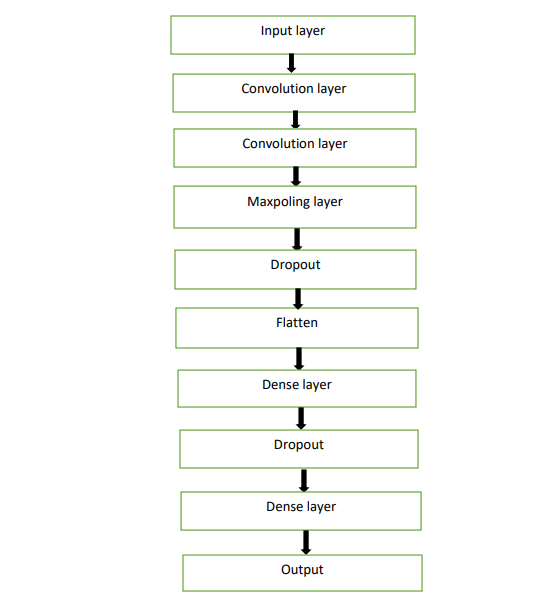
\includegraphics[width=\linewidth]{475f.png}
        \caption{CNN layers}
        \label{fig:CNN_Layers}
    \end{figure}
\end{center}


\begin{itemize}
\item \textbf{Input Layer: } For input of our CNN at first, we reshaped our images to 48x48 pixel size.
\item \textbf{Convolution Layer 1:}  In this layer inputs are 48x48 pixel size. In this layer, we use 32 kernels and each kernel size is 3x3  and strides size is 1x1 means each kernel traverses the full image by increasing 1 row or 1 column. For activation, we use RELU (max(x,0)) for this layer.
\item \textbf{Convolution Layer 2:} In this layer, the input comes from Convolution layer 1. In this layer, we used 64 kernels and the kernel size and strides size are the same as the Convolution layer 1. For activation, we use RELU (max(x,0)) for this layer.
\item \textbf{Max pooling layer:} In this layer, we used a pooling matrix size of 2x2. In this layer strides size is 2x2 means the pooling matrix traverses the full matrix that comes from convolution layer 2  by increasing 2 rows or 2 columns. 
\item \textbf{Dropout: } To reduce overfitting we dropped out some connections. In our project, we dropped out 25\% of connections. 
\item \textbf{Flatten:} For this layer, we need to reshape our matrix 2 dimensional to 1 dimensional. To reshape our matrix comes from the pooling layer we use this layer.
\item \textbf{Dense Layer 1: } In this layer, images are partially classified. In this layer, we used RELU( max(x,0) ) as an activation function for the next layer. And in the next layer, our number of hidden nodes is 1024. So we also needed to define this.
\item \textbf{Dropout: }To reduce overfitting again we dropped out some connections. In our project, we dropped out 25\% of connections.
\item \textbf{Dense Layer 2: } This is the final layer for our project.  In this layer, images are fully classified. In this layer, we used softmax as an activation function for the next layer. Since we worked on 7 emotions so we needed to define this as the number of nodes in the next layer. 

\end{itemize}

In our project, we used a learning rate of 0.1\%.  To train our model we used 64 as batch size means for each run we used 64 images to train our model. And for this every iteration our CNN runs 448 times and finally, we use 30 iterations for better accuracy. 

To predict emotion our model gets an input of an image with a human face and the size is 48x48. For this we used OpenCV. By using OpenCV “haar cascade frontal face default” classifier to detect human face and then we cropped this portion and resized it to 48x48 pixel and sent it to our trained model to predict the emotion from this image. For time complexity we used a Grayscale image for all of our procedures. So before sending an image for predicting we also converted it to a grayscale image. 


\section{Implementation}
\subsection{Data Collection:}
We collected the dataset from kaggle.com. This is the web link\cite{FER2013K4:online} we collected our dataset for completing our project. This dataset contains 28709 train image data and 7178 test images. 

\subsection{Data Processing:}
Since we collected data from Kaggle so don’t need to process our dataset. 
\subsection{Model Development}
For developing our model we use the Python programming language. For video capturing we used Python OpenCV and to train our model, we used Keras, a Machine learning API of Python. To bring the dataset from the directory we used the Imagegenerator function of Keras. We used batch size 64 for each time of run algorithm that gives 64 images from our dataset. 

\subsection{Results}
After training our model we saw the accuracy of our model is 98\%. We saved the data of our model in a model.h5 file because to train our model it takes too much time. To predict emotions in video streaming we used this file to load our model. 



\section{Conclusion}
\subsection{Challenges:}
While completing our project there are some sectors of the project we faced challenges. One of them is building a neural network. To be more precise, determining the numbers of hidden layers in the conventional neural network was a bit challenging for us. As there are different types of layers and each has its own work. So determining them was a bit hard.
Another sector where we faced challenges is crop the image we received from OpenCV. As we receive a full image from the OpenCV face being detected. So after receiving it we have cropped the image while maintaining the pixel size and use our model on it to determine the expression.
Apart from these problems we also faced the challenge of choosing the trained model. As the trained model should not be overfitted. If the trained model is overfitted it will have a negative impact on the project as it will affect the model’s ability to generalize as well as to work with new data. So we had to carefully choose the trained model of our project.   

\subsection{Limitations:}
There are some limitations to our project. But the one which needs to be explained is the inability to replace the human face with emoji.  As we wanted to determine the facial emotion and replace it with similar emotion-based emoji. But it was difficult for us to build the emoji and replace it with the face. So we only determined the facial emotion.

\subsection{Future directions:}
So using our project the live streaming and face timing apps can maintain the users’ privacy. As people are not comfortable facing the camera and so also do not want to reveal their true identity. Because of this problem they do not come out of their shell while being very talented. So using the system they can simply hide their face replacing it with the emoji and keep their identity a secret as long as they please or comfortable to reveal their true identity.


\bibliographystyle{plain}
\bibliography{references}

\end{document}
